\documentclass[a4paper, 11pt]{article}

% packages
\usepackage[utf8]{inputenc}
\usepackage{amsmath}
\usepackage{amsfonts}
\usepackage{array}
\usepackage{booktabs}
\usepackage{chngcntr}
\usepackage{colortbl}
\usepackage{dcolumn}
\usepackage{floatrow}
\usepackage{geometry}
\usepackage{graphicx}
\usepackage{hyperref}
\usepackage{multirow}
\usepackage{natbib}
\usepackage[normalem]{ulem}
\usepackage{ntheorem}
\usepackage{pdflscape}
\usepackage{rotating}
\usepackage{setspace}
\usepackage{subfigure}
\usepackage{tabularx}
\usepackage{threeparttable}
\usepackage[numbib, nottoc, notlot, notlof]{tocbibind}
\usepackage{wrapfig}
\usepackage{xcolor}

% page styling
\geometry{
  a4paper,
  left=1in,
  right=1in,
  bottom=1.2in,
  top=1.2in
}
\pagestyle{plain}
\pagenumbering{arabic}
\linespread{1.5}
\hypersetup{
  colorlinks,
  linkcolor={red!50!black},
  citecolor={blue!50!black},
  urlcolor={blue!80!black}
}
\theoremseparator{:}
\newtheorem{hyp}{Hypothesis}
\counterwithin*{hyp}{section}

\renewcommand{\thefootnote}{\fnsymbol{footnote}}

\title{
	Party Nomination Strategy and its Representational Consequences in Interactive Mixed-Member Majoritarian Systems
	\footnotemark{}
	\footnotetext[1]{This paper was previously entitled and circulated as ``Youth Underrepresentation and Parties' Nomination Strategy in Mixed-Member Electoral Systems". Earlier versions of this paper were presented at the 2024 summer meeting of the Japanese Society for Quantitative Political Science (JSQPS) and 2024 Annual Meeting of Americal Political Science Association (APSA). I thank Dan Smith for sharing the latest version of his data, and Serika Atsumi, Yuki Atsusaka, Amy Catalinac, Kentaro Fukumoto, Yusaku Horiuchi, Junko Kato, Kenneth McElwain, Mayuko Toba, Masahiro Yamada, Hironao Yoda for their comments.}
}

\author{
	Dai Sasaki
	\thanks{Master's Student, Graduate Schools for Law and Politics, The University of Tokyo. Email: daichansama12@g.ecc.u-tokyo.ac.jp; Website: https://dxxsxsxkx.github.io.}
}

\date{
	First Version: 28 Jun, 2024 \\
	This Version: 6 Dec, 2024 
}

\begin{document}

\maketitle

\renewcommand{\thefootnote}{\arabic{footnote}}
\setcounter{footnote}{0}

\begin{abstract} 
I argue that interactive mixed-member majoritarian systems (interactive MMMs), a variant of mixed member systems where parties can nominate the same candidates in both majoritarian and proportional representation (PR) tiers (dual listing), diminish the representational advantages commonly associated with PR systems. Analyzing comprehensive, candidate-level data of Japan's lower house elections, I show that parties give higher list ranks to senior candidates, incumbents, and dual-listed candidates. Furthermore, incumbents are more likely to be dual-listed than non-incumbents. These patterns apply across parties, but are less applicable to situations of intra-party disputes and government transitions, where seniors and incumbents may give their way to newcomers. My analysis suggests that interactive MMMs sustain representational inequalities between groups by reducing the electoral prospects of newcomers and making legislative turnover less frequent.
\end{abstract}

\newpage

\section{Introduction}

% TODO: write

\section{Theory} \label{sec: the}

\subsection{Theoretical Expectations}

% TODO: write

\subsection{Case: Japan's Mixed-Member Majoritarian System}

% TODO: write

\begin{figure}[!htbp]
	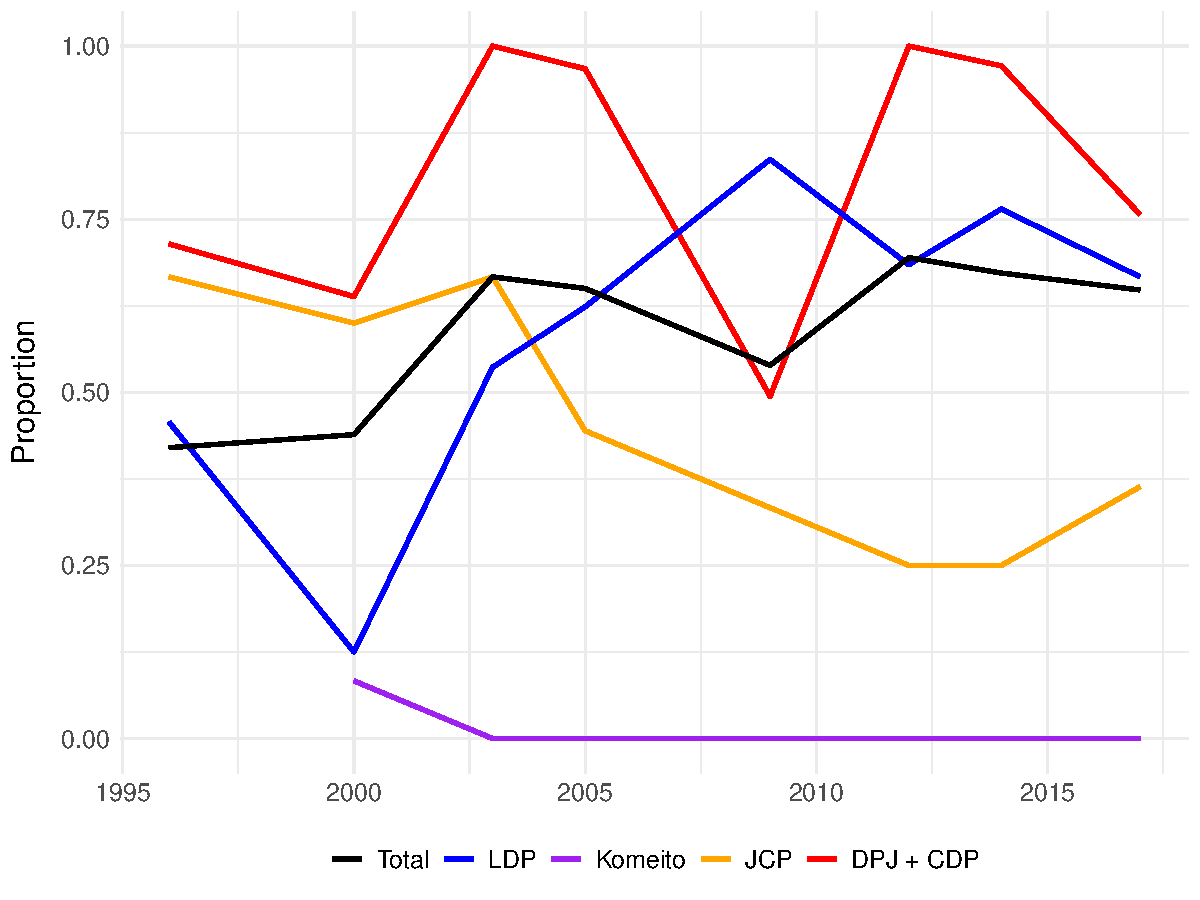
\includegraphics[width = 0.9\textwidth]{../figure/paper/dual_nomination.pdf}
	\caption{Share of Dual-Listed Candidates among PR Winners}
	\label{fig:dual}
\end{figure}

% created manually
\begin{table}[!htbp]
\centering
\begin{threeparttable}
\begin{tabular}{cccccccccc}
\toprule
\multicolumn{8}{c}{Valid} & \multicolumn{2}{c}{Invalid} \\
\cmidrule(lr){1-8} \cmidrule(lr){9-10}
\multicolumn{2}{c}{List A} & \multicolumn{2}{c}{List B} & \multicolumn{2}{c}{List C} & \multicolumn{2}{c}{List D} & \multicolumn{2}{c}{List E} \\
\cmidrule(lr){1-2} \cmidrule(lr){3-4} \cmidrule(lr){5-6} \cmidrule(lr){7-8} \cmidrule(lr){9-10}
Rank & Dual & Rank & Dual & Rank & Dual & Rank & Dual & Rank & Dual \\
\cmidrule(lr){1-2} \cmidrule(lr){3-4} \cmidrule(lr){5-6} \cmidrule(lr){7-8} \cmidrule(lr){9-10}
1 & - & 1 & - & 1 & \checkmark & 1 & \checkmark & 1 & - \\
2 & - & 2 & \checkmark & 1 & \checkmark & 1 & \checkmark & 1 & - \\
3 & - & 2 & \checkmark & 1 & \checkmark & 3 & \checkmark & 3 & - \\
4 & - & 2 & \checkmark & 1 & \checkmark & 3 & \checkmark & 4 & \checkmark \\
5 & - & 2 & \checkmark & 5 & - & 5 & - & 5 & \checkmark \\
6 & - & 6 & \checkmark & 6 & - & 6 & - & 6 & - \\
7 & - & 7 & \checkmark & 7 & - & 7 & - & 7 & - \\
8 & - & 8 & \checkmark & 8 & - & 8 & - & 8 & - \\
\bottomrule
\end{tabular}
\begin{tablenotes}[flushleft]
  \scriptsize{
    \item \textit{Note.} This table presents five hypothetical party lists that may be submitted in the PR tier of Japan's mixed member majoritarian system. Dual-listed candidates are denoted by \checkmark. Lists A, B, C, and D are all valid. List E is invalid, as pure-PR candidates cannot be ranked equal. 
  }
\end{tablenotes}
\end{threeparttable}
\caption{Valid and Invalid List Structures in Japan's Interactive MMM system}
\label{tab:listStructure}
\end{table}



















\section{Data and Method} \label{sec: emp}

% TODO: write

\section{Result} \label{sec: res}

\subsection{Aggregate-Level Analysis}

% TODO: write

\begin{figure}[!htbp]
	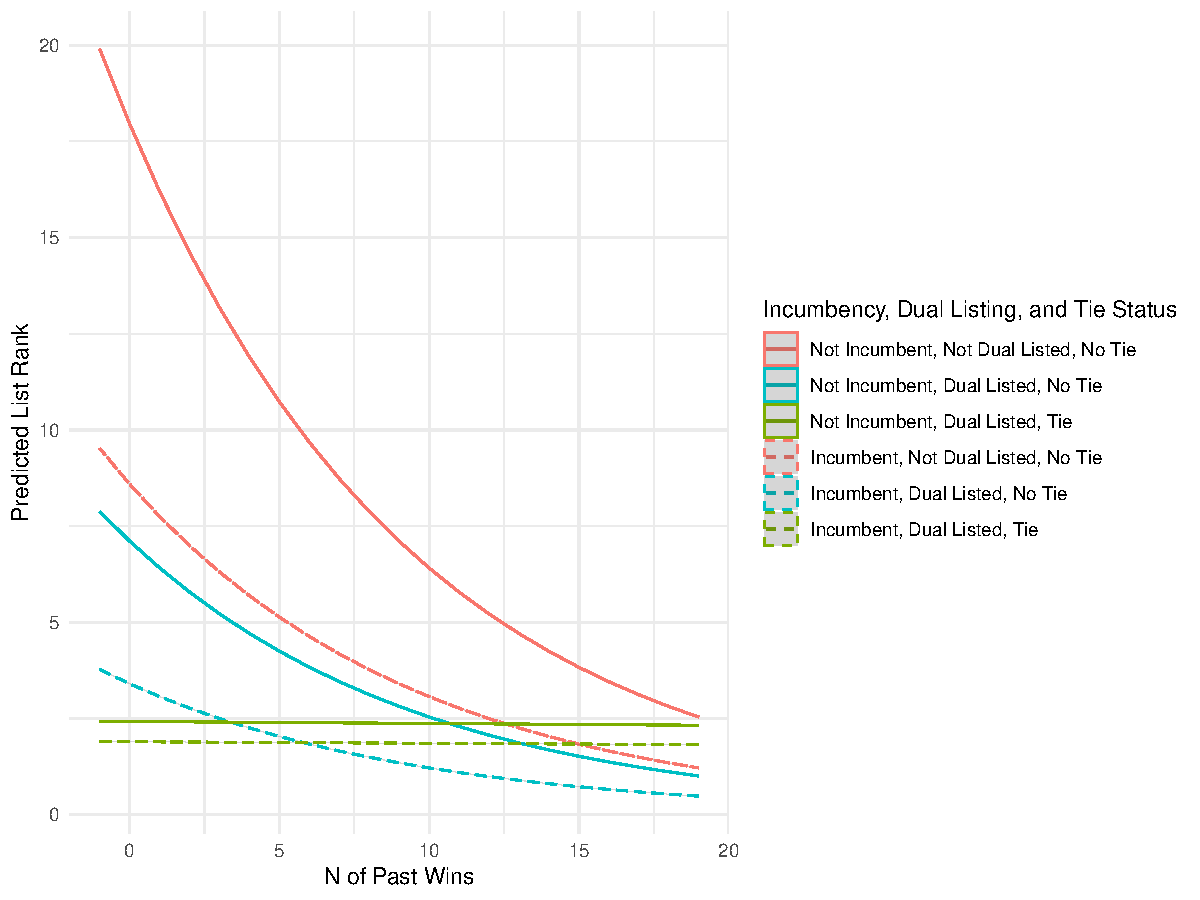
\includegraphics[width = 0.9\textwidth]{../figure/paper/marginal_effects_rank.pdf}
	\caption{Marginal Effects of Seniority, Incumbency, Dual Listing, and Tie Status on List Rank}
	\label{fig:marginal_rank}
\end{figure}

\begin{figure}[!htbp]
	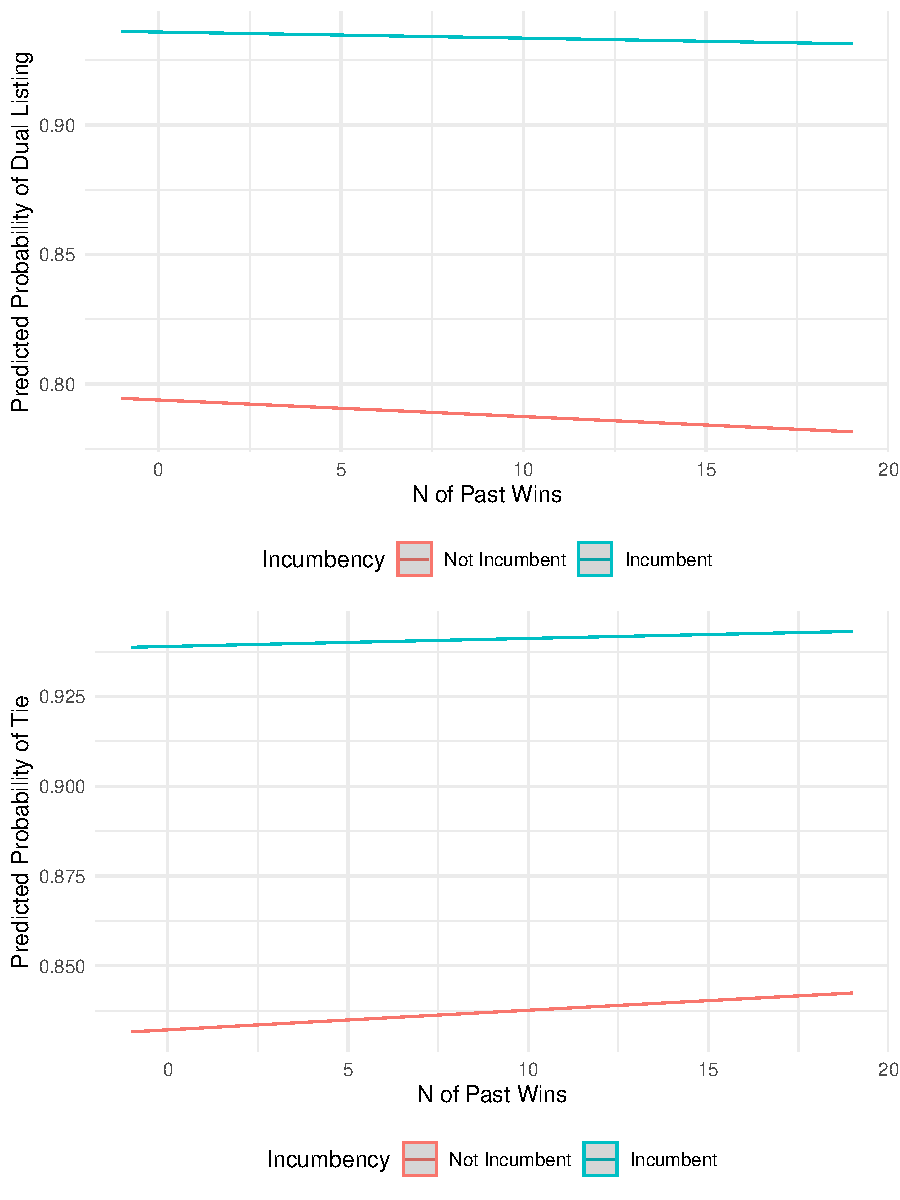
\includegraphics[width = 0.9\textwidth]{../figure/paper/marginal_effects_dual_tie.pdf}
	\caption{Marginal Effects of Seniority and Incumbency on Dual Listing}
	\label{fig:marginal_dual}
\end{figure}


\subsection{Party-Specific Analysis}

% TODO: write


\begin{table}[!htbp]
\begin{center}
\scalebox{0.6}{
\begin{threeparttable}
\begin{tabular}{l D{.}{.}{5.5} D{.}{.}{5.5} D{.}{.}{5.5} D{.}{.}{5.5} D{.}{.}{5.5} D{.}{.}{5.5} D{.}{.}{5.5} D{.}{.}{5.5} D{.}{.}{5.5} D{.}{.}{5.5}}
\toprule
 & \multicolumn{4}{c}{List Rank} & \multicolumn{3}{c}{Dual Listing} & \multicolumn{3}{c}{Dual Listing (Tie)} \\
\cmidrule(lr){2-5} \cmidrule(lr){6-8} \cmidrule(lr){9-11}
 & \multicolumn{1}{c}{Model 1} & \multicolumn{1}{c}{Model 2} & \multicolumn{1}{c}{Model 3} & \multicolumn{1}{c}{Model 4} & \multicolumn{1}{c}{Model 5} & \multicolumn{1}{c}{Model 6} & \multicolumn{1}{c}{Model 7} & \multicolumn{1}{c}{Model 8} & \multicolumn{1}{c}{Model 9} & \multicolumn{1}{c}{Model 10} \\
\midrule
Total Wins         & -0.15^{***}             &                         &                         & -0.14^{***}             & 0.19^{***}              &                         & 0.01                    & 0.19^{***}              &                         & 0.02                    \\
                   & (0.01)                  &                         &                         & (0.01)                  & (0.02)                  &                         & (0.02)                  & (0.02)                  &                         & (0.02)                  \\
Incumbency         &                         & -1.26^{***}             &                         & -0.87^{***}             &                         & 1.64^{***}              & 1.65^{***}              &                         & 1.60^{***}              & 1.57^{***}              \\
                   &                         & (0.04)                  &                         & (0.07)                  &                         & (0.11)                  & (0.14)                  &                         & (0.11)                  & (0.14)                  \\
Dual Listing       &                         &                         & -2.00^{***}             & -1.52^{***}             &                         &                         &                         &                         &                         &                         \\
                   &                         &                         & (0.03)                  & (0.13)                  &                         &                         &                         &                         &                         &                         \\
Tie                &                         &                         &                         & -3.27^{***}             &                         &                         &                         &                         &                         &                         \\
                   &                         &                         &                         & (0.66)                  &                         &                         &                         &                         &                         &                         \\
Female             &                         &                         &                         & -0.17^{**}              &                         &                         & -0.58^{**}              &                         &                         & -0.70^{***}             \\
                   &                         &                         &                         & (0.05)                  &                         &                         & (0.18)                  &                         &                         & (0.17)                  \\
Block Magnitude    &                         &                         &                         & 0.01^{***}              &                         &                         & 0.05^{***}              &                         &                         & 0.05^{***}              \\
                   &                         &                         &                         & (0.00)                  &                         &                         & (0.01)                  &                         &                         & (0.01)                  \\
Total Wins x Tie   &                         &                         &                         & 0.14^{***}              &                         &                         &                         &                         &                         &                         \\
                   &                         &                         &                         & (0.01)                  &                         &                         &                         &                         &                         &                         \\
Tie x Incumbency   &                         &                         &                         & 0.71^{***}              &                         &                         &                         &                         &                         &                         \\
                   &                         &                         &                         & (0.08)                  &                         &                         &                         &                         &                         &                         \\
Tie x Dual Listing &                         &                         &                         & 2.51^{***}              &                         &                         &                         &                         &                         &                         \\
                   &                         &                         &                         & (0.67)                  &                         &                         &                         &                         &                         &                         \\
\midrule
Year FE            & \multicolumn{1}{c}{Yes} & \multicolumn{1}{c}{Yes} & \multicolumn{1}{c}{Yes} & \multicolumn{1}{c}{Yes} & \multicolumn{1}{c}{Yes} & \multicolumn{1}{c}{Yes} & \multicolumn{1}{c}{Yes} & \multicolumn{1}{c}{Yes} & \multicolumn{1}{c}{Yes} & \multicolumn{1}{c}{Yes} \\
Party FE           & \multicolumn{1}{c}{No}  & \multicolumn{1}{c}{No}  & \multicolumn{1}{c}{No}  & \multicolumn{1}{c}{No}  & \multicolumn{1}{c}{No}  & \multicolumn{1}{c}{No}  & \multicolumn{1}{c}{No}  & \multicolumn{1}{c}{No}  & \multicolumn{1}{c}{No}  & \multicolumn{1}{c}{No}  \\
AIC                & 16370.59                & 15871.58                & 14270.41                & 13692.05                & 2639.55                 & 2491.96                 & 2442.14                 & 2712.74                 & 2572.15                 & 2513.64                 \\
BIC                & 16436.29                & 15937.28                & 14336.11                & 13805.53                & 2699.27                 & 2551.68                 & 2519.78                 & 2772.47                 & 2631.88                 & 2591.28                 \\
Log Likelihood     & -8174.30                & -7924.79                & -7124.21                & -6827.03                & -1309.77                & -1235.98                & -1208.07                & -1346.37                & -1276.08                & -1243.82                \\
Deviance           & 2920.43                 & 2822.00                 & 2377.49                 & 2344.53                 & 2619.55                 & 2471.96                 & 2416.14                 & 2692.74                 & 2552.15                 & 2487.64                 \\
Num. obs.          & 2900                    & 2900                    & 2900                    & 2900                    & 2900                    & 2900                    & 2900                    & 2900                    & 2900                    & 2900                    \\
\bottomrule
\end{tabular}
\begin{tablenotes}[flushleft]
\scriptsize{\item $^{***}p<0.001$; $^{**}p<0.01$; $^{*}p<0.05$. Standard errors in parentheses.
\item Dependent variable: candidate $i$'s list rank (columns 1-4) dual listing status (columns 5-7), and whether the candidate has a tie on the list (columns 8-10).
\item Estimated models: negatige binomial (columns 1-4) and logit (columns 5-10).}
\end{tablenotes}
\end{threeparttable}
}
\caption{Regression Results for LDP Candidates}
\label{tab:ldp}
\end{center}
\end{table}



\begin{table}[!bth]
\begin{center}
\begin{threeparttable}
\begin{tabular}{l D{.}{.}{4.5} D{.}{.}{4.5} D{.}{.}{5.5} D{.}{.}{5.5} D{.}{.}{5.5}}
\toprule
 & \multicolumn{2}{c}{Dual Listing} & \multicolumn{3}{c}{List Rank} \\
\cmidrule(lr){2-3} \cmidrule(lr){4-6}
 & \multicolumn{1}{c}{H1} & \multicolumn{1}{c}{H2} & \multicolumn{1}{c}{H3} & \multicolumn{1}{c}{H4} & \multicolumn{1}{c}{H5} \\
\midrule
Total Wins      & 0.35^{***}              &                         & -0.14^{***}             &                         &                         \\
                & (0.07)                  &                         & (0.01)                  &                         &                         \\
Incumbency      &                         & 1.25^{***}              &                         & -0.74^{***}             &                         \\
                &                         & (0.24)                  &                         & (0.06)                  &                         \\
Dual Listing    &                         &                         &                         &                         & -2.53^{***}             \\
                &                         &                         &                         &                         & (0.05)                  \\
Female          & -0.04                   & -0.11                   & -0.00                   & -0.02                   & -0.01                   \\
                & (0.24)                  & (0.24)                  & (0.08)                  & (0.08)                  & (0.06)                  \\
Block Magnitude & 0.04^{**}               & 0.04^{**}               & 0.01^{**}               & 0.01^{***}              & 0.02^{***}              \\
                & (0.01)                  & (0.01)                  & (0.00)                  & (0.00)                  & (0.00)                  \\
\midrule
Year FE         & \multicolumn{1}{c}{Yes} & \multicolumn{1}{c}{Yes} & \multicolumn{1}{c}{Yes} & \multicolumn{1}{c}{Yes} & \multicolumn{1}{c}{Yes} \\
Party FE        & \multicolumn{1}{c}{Yes} & \multicolumn{1}{c}{Yes} & \multicolumn{1}{c}{Yes} & \multicolumn{1}{c}{Yes} & \multicolumn{1}{c}{Yes} \\
AIC             & 949.35                  & 951.02                  & 8026.35                 & 7974.18                 & 6423.06                 \\
BIC             & 1010.13                 & 1011.79                 & 8092.65                 & 8040.48                 & 6489.36                 \\
Log Likelihood  & -463.68                 & -464.51                 & -4001.17                & -3975.09                & -3199.53                \\
Deviance        & 927.35                  & 929.02                  & 1608.56                 & 1589.41                 & 1033.39                 \\
Num. obs.       & 1854                    & 1854                    & 1854                    & 1854                    & 1854                    \\
\bottomrule
\end{tabular}
\begin{tablenotes}[flushleft]
\scriptsize{\item $^{***}p<0.001$; $^{**}p<0.01$; $^{*}p<0.05$. Standard errors in parentheses.
\item Dependent variable: candidate $i$'s list rank (H1-2) and dual nomination status (H3-5).
\item Estimated models: logit (H1-2) and negative binomial (H3-5).}
\end{tablenotes}
\end{threeparttable}
\caption{Regression Results for DPJ / CDP Candidates}
\label{tab:regDPJCDP}
\end{center}
\end{table}


\subsection{Election- / Party-Specific Analysis}


\begin{table}
\begin{center}
\begin{tabular}{l c c c c c}
\hline
 & \multicolumn{3}{c}{2005} & \multicolumn{2}{c}{2012} \\
\cline{2-4} \cline{5-6}
 & List Rank & Dual Listing & Tie & List Rank & Dual Listing \\
\hline
Total Wins         & $-0.01$       & $0.03$       & $0.06$       & $0.02$        & $0.61^{*}$   \\
                   & $(0.02)$      & $(0.09)$     & $(0.08)$     & $(0.04)$      & $(0.25)$     \\
Incumbency         & $-2.03^{***}$ & $1.76^{***}$ & $1.47^{***}$ & $-0.23$       & $1.48$       \\
                   & $(0.16)$      & $(0.46)$     & $(0.42)$     & $(0.28)$      & $(1.21)$     \\
Dual Listing       & $-1.77^{***}$ &              &              & $-3.41^{***}$ &              \\
                   & $(0.17)$      &              &              & $(0.09)$      &              \\
Tie                & $-3.26^{**}$  &              &              &               &              \\
                   & $(1.01)$      &              &              &               &              \\
Female             & $-0.56^{***}$ & $0.52$       & $-0.31$      & $-0.06$       & $0.57$       \\
                   & $(0.10)$      & $(0.59)$     & $(0.48)$     & $(0.12)$      & $(0.69)$     \\
Block Magnitude    & $0.04^{***}$  & $0.04$       & $0.05^{*}$   & $0.04^{***}$  & $0.10^{***}$ \\
                   & $(0.00)$      & $(0.02)$     & $(0.02)$     & $(0.00)$      & $(0.03)$     \\
Total Wins x Tie   & $0.01$        &              &              &               &              \\
                   & $(0.02)$      &              &              &               &              \\
Tie x Incumbency   & $2.00^{***}$  &              &              &               &              \\
                   & $(0.18)$      &              &              &               &              \\
Tie x Dual Listing & $3.11^{**}$   &              &              &               &              \\
                   & $(1.02)$      &              &              &               &              \\
\hline
Year FE            & Yes           & Yes          & Yes          & Yes           & Yes          \\
Party FE           & No            & No           & No           & No            & No           \\
AIC                & $1418.21$     & $276.68$     & $310.14$     & $910.24$      & $227.80$     \\
BIC                & $1460.19$     & $295.77$     & $329.23$     & $944.33$      & $246.73$     \\
Log Likelihood     & $-698.10$     & $-133.34$    & $-150.07$    & $-446.12$     & $-108.90$    \\
Deviance           & $228.28$      & $266.68$     & $300.14$     & $84.16$       & $217.80$     \\
Num. obs.          & $336$         & $336$        & $336$        & $326$         & $326$        \\
\hline
\multicolumn{6}{l}{\scriptsize{\item $^{***}p<0.001$; $^{**}p<0.01$; $^{*}p<0.05$. Standard errors in parentheses.
\item Dependent variable: candidate $i$'s list rank (columns 1 / 3) dual listing status (columns 2 / 4), and whether the candidate has a tie on the list (columns 3 / 6).
\item Estimated models: negatige binomial (columns 1 / 4) and logit (columns 2-3, 5-6). 
\textit{Note.} All dual-listed LDP candidates in the 2012 general election had ties on the list.}}
\end{tabular}
\caption{Regression Results for LDP Candidates in 2005 and 2012}
\label{tab:ldp_2005_2012}
\end{center}
\end{table}


% TODO: write

\section{Discussion} \label{sec: dis}

% TODO: write

\subsection{Legislative Turnover}

% TODO: write

\subsection{Representation}

% TODO: write

\begin{table}[htbp]
\begin{center}
\begin{threeparttable}
% latex table generated in R 4.1.0 by xtable 1.8-4 package
% NOTE: manually modified on 27 Nov 2023. 
% Sat Jul  8 06:31:47 2023
\begin{tabular}{lccccc}
\toprule
Country & Eligibility & Average & \% U30 & \% U40 & \% U45 \\ 
\midrule
Canada & 18 & 50 & 1.95 & 16.88 & 30.19 \\ 
France & 18 & 49 & 4.85 & 26.52 & 37.95 \\ 
Germany & 18 & 47 & 8.83 & 28.94 & 41.98 \\ 
Italy & 25 & 49 & 1.25 & 16.25 & 35 \\ 
Japan & 25 & 55 & 0.22 & 6.02 & 17.2 \\ 
UK & 18 & 51 & 3.69 & 21.69 & 34 \\ 
USA & 25 & 57 & 0.46 & 10.42 & 20.14 \\ 
\bottomrule
\end{tabular}

\begin{tablenotes}[flushleft]
  \scriptsize{
    \item{\textit{Note.} Age demographics of lower house members in the G7 countries, as of January 2023. Eligibility is the minimum age to run for the house.}
    \item{\textit{Source.} \citet{inter-parliamentaryunionDataAgeCountry2024}.}
  }
\end{tablenotes}
\end{threeparttable}
\caption{Age Demographics of Lower Houses in the G7 Countries}
\label{table:intl}
\end{center}
\end{table}


% created manually, based on prepCareer.Rmd
% for each general election, display: 
% mean age of those elected for the first time
% number of those elected for the first time
% proportion of such candidates

\begin{table}[ht]
\begin{threeparttable}
\begin{tabular}{c|ccccccccc}
\toprule
Year & 1947 & 1949 & 1952 & 1953 & 1955 & 1958 & 1960 & 1963 & 1967 \\
\midrule
Mean age & 48.7 & 47.4 & 54.6 & 52.3 & 52.2 & 49.0 & 48.4 & 47.1 & 46.1 \\
Proportion & 1.00 & 0.47 & 0.44 & 0.15 & 0.16 & 0.15 & 0.13 & 0.15 & 0.21 \\
Mean age (all) & 48.7 & 48.6 & 52.8 & 52.6 & 53.9 & 54.6 & 55.6 & 56.1 & 56.2 \\
\midrule 
Year & 1969 & 1972 & 1976 & 1979 & 1980 & 1983 & 1986 & 1990 & 1993 \\
\midrule 
Mean age & 45.3 & 47.8 & 48.0 & 49.0 & 45.2 & 48.7 & 48.4 & 48.9 & 44.1 \\
Proportion & 0.19 & 0.19 & 0.25 & 0.15 & 0.07 & 0.17 & 0.13 & 0.26 & 0.26 \\
Mean age (all) & 55.1 & 55.3 & 55.0 & 55.8 & 56.1 & 56.0 & 56.9 & 56.4 & 54.3 \\
\midrule 
Year & 1996 & 2000 & 2003 & 2005 & 2009 & 2012 & 2014 & 2017 \\
\midrule 
Mean age & 48.7 & 46.4 & 44.5 & 44.4 & 46.3 & 44.8 & 47.2 & 47.7 \\
Proportion & 0.24 & 0.22 & 0.22 & 0.21 & 0.33 & 0.38 & 0.09 & 0.12 \\
Mean age (all) & 55.2 & 54.6 & 53.1 & 52.4 & 52.2 & 51.9 & 53.0 & 54.7 \\
\bottomrule
\end{tabular}
\begin{tablenotes}[flushleft]
  \scriptsize{
    \item Mean age and proportion of MPs elected for the first time, and mean age of All MPs elected in each general election. 
    \item \textit{Data source}: Reed and Smith (2017)
  }
\end{tablenotes}
\end{threeparttable}
\caption{Data of First-Time Winners}
\label{table:firstElection}
\end{table}


\begin{figure}[!htbp]
	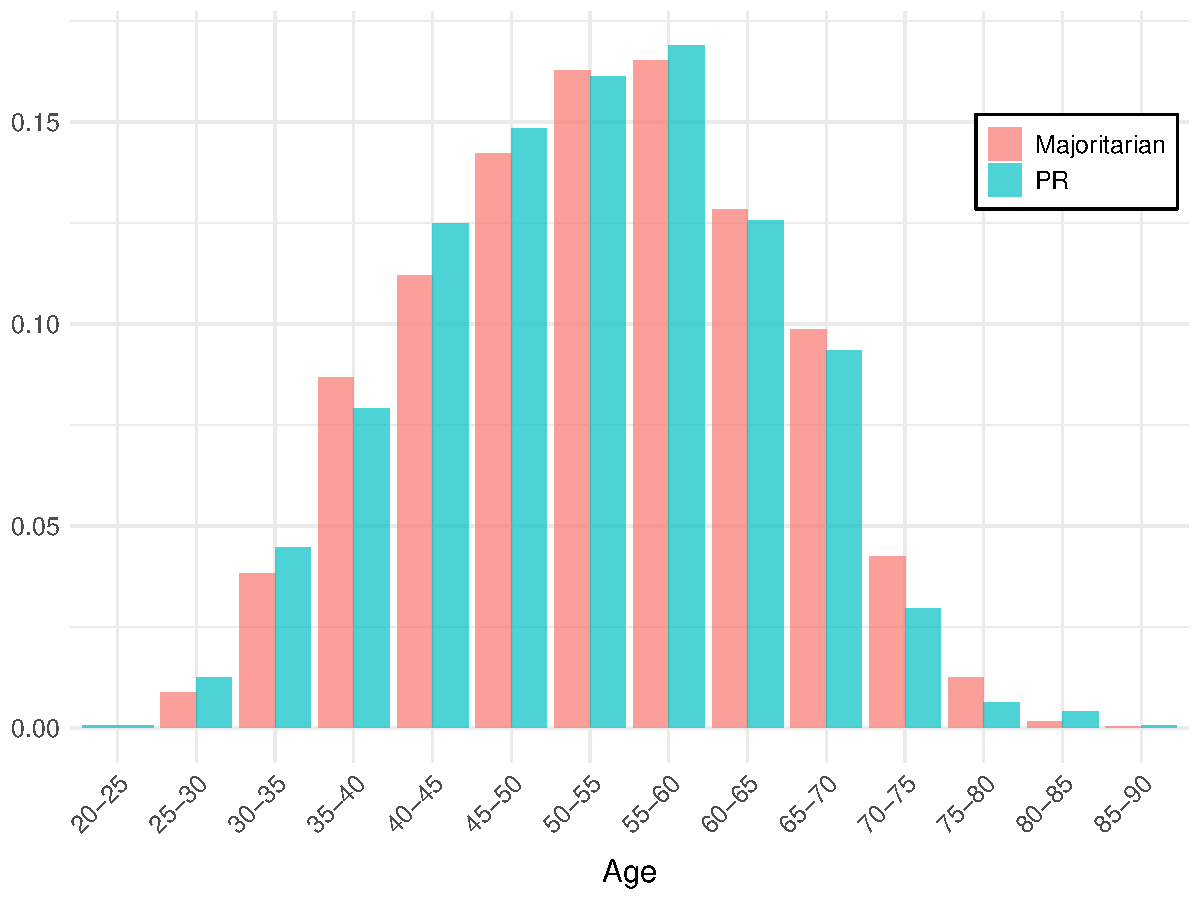
\includegraphics[width = 0.9\textwidth]{../figure/paper/age_smd_vs_pr_winners.pdf}
	\caption{Age Composition of Legislators Elected from the Two Tiers}
	\label{fig:pr_vs_smd}
\end{figure}



\begin{figure}[!htbp]
	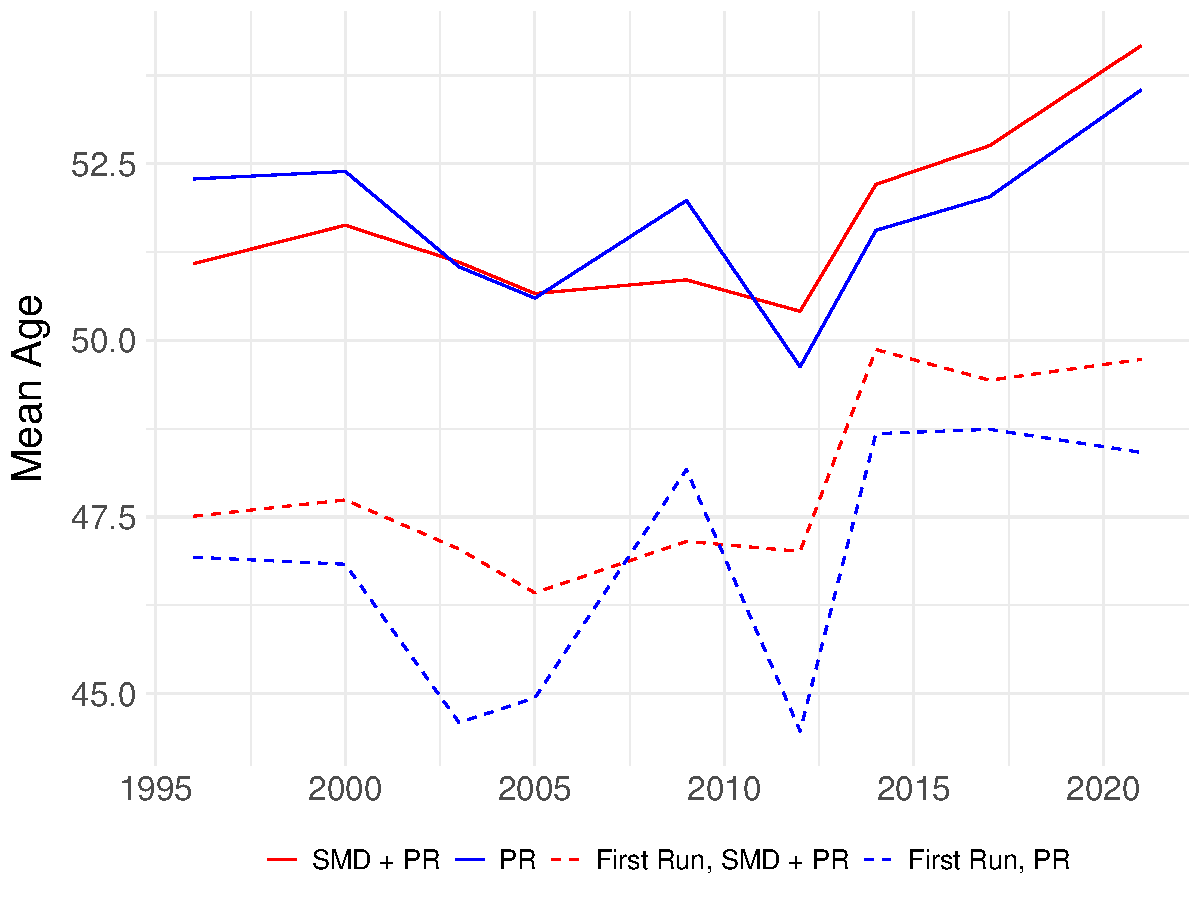
\includegraphics[width = 0.9\textwidth]{../figure/paper/age_first_run.pdf}
	\caption{Age Comparison: Average vs. New Candidates}
	\label{fig:ageFirstRun}
\end{figure}



\section{Conclusion}

% TODO: write

\newpage

\bibliography{../bibliography.bib}
\bibliographystyle{apalike}

\newpage

\appendix

\setcounter{table}{0}
\setcounter{figure}{0}
\renewcommand{\thetable}{A\arabic{table}}
\renewcommand{\thefigure}{A\arabic{figure}}

\section{Summary Statistics}

\subsection{Candidate-Level Summary Statistics}

% TODO: add a revised table
\begin{table}[!htbp] \centering \renewcommand*{\arraystretch}{1.1}\caption{Summary Statistics}\resizebox{\textwidth}{!}{
\begin{threeparttable}
\begin{tabular}{l|cccccccc}
\toprule
Variable & N & Mean / \% & Std. Dev. & Min & \% 25 & \% 50 & \% 75 & Max \\ 
\midrule
Gender & 6935 &  &  &  &  &  &  &  \\ 
... Female & 881 & 12.7\% &  &  &  &  &  &  \\ 
... Male & 6054 & 87.3\% &  &  &  &  &  &  \\ 
N of wins before & 6935 & 1.776 & 2.487 & 0 & 0 & 1 & 3 & 19 \\ 
Incumbency & 6935 &  &  &  &  &  &  &  \\ 
... Incumbent & 3129 & 45.1\% &  &  &  &  &  &  \\ 
... Non-Incumbent & 3806 & 54.9\% &  &  &  &  &  &  \\ 
List Rank & 6935 & 4.317 & 6.976 & 1 & 1 & 2 & 4 & 52\\ 
Dual Listing & 6935 &  &  &  &  &  &  &  \\ 
... Yes & 5292 & 76.3\% &  &  &  &  &  &  \\ 
... No & 1643 & 23.7\% &  &  &  &  &  &  \\ 
\bottomrule
\end{tabular}
\begin{tablenotes}[flushleft]
  \scriptsize{
    \item Candidate-level summary statistics. 
    \item \textit{Data source}: \citet{reedsmith2018} 
  }
\end{tablenotes}
\end{threeparttable}
}
\label{tab:stats}
\end{table}



\newpage

\subsection{Magnitudes of PR Blocks, 1996 - 2021}

% created manually
\begin{table}[!htbp]
\begin{threeparttable}
\begin{tabular}{lccccccccc}
\toprule
Bloc & 1996 & 2000 & 2003 & 2005 & 2009 & 2012 & 2014 & 2017 & 2021 \\
\midrule
Hokkaido & 9 & 8 & 8 & 8 & 8 & 8 & 8 & 8 & 8 \\
Tohoku & 16 & 14 & 14 & 14 & 14 & 14 & 14 & 13 & 13 \\
Kita-kanto & 21 & 20 & 20 & 20 & 20 & 20 & 20 & 19 & 19 \\
Tokyo & 19 & 17 & 17 & 17 & 17 & 17 & 17 & 17 & 17 \\
Minami-kanto & 23 & 21 & 22 & 22 & 22 & 22 & 22 & 22 & 22 \\
Hokuriku Shinetsu & 13 & 11 & 11 & 11 & 11 & 11 & 11 & 11 & 11 \\
Tokai & 23 & 21 & 21 & 21 & 21 & 21 & 21 & 21 & 21 \\
Kinki & 33 & 30 & 30 & 30 & 29 & 29 & 29 & 28 & 28 \\
Chugoku & 13 & 11 & 11 & 11 & 11 & 11 & 11 & 11 & 11 \\
Shikoku & 7 & 6 & 6 & 6 & 6 & 6 & 6 & 6 & 6 \\
Kyushu & 23 & 21 & 21 & 21 & 21 & 21 & 21 & 20 & 20 \\
\bottomrule
\end{tabular}
\begin{tablenotes}[flushleft]
  \scriptsize{
    \item Magnitudes of each PR regional district for elections 1996 - 2021. 
    \item \textit{Data source}: \citet{reedReedSmithJapaneseHouse2017, ministryofinternalaffairsandcommunicationsElectionSenkyo2024}
  }
\end{tablenotes}
\end{threeparttable}
\caption{Magnitudes of PR Blocks}
\label{tab:distM}
\end{table}

\newpage

\subsection{Distribution of List Rank}

\begin{figure}[!htbp]
	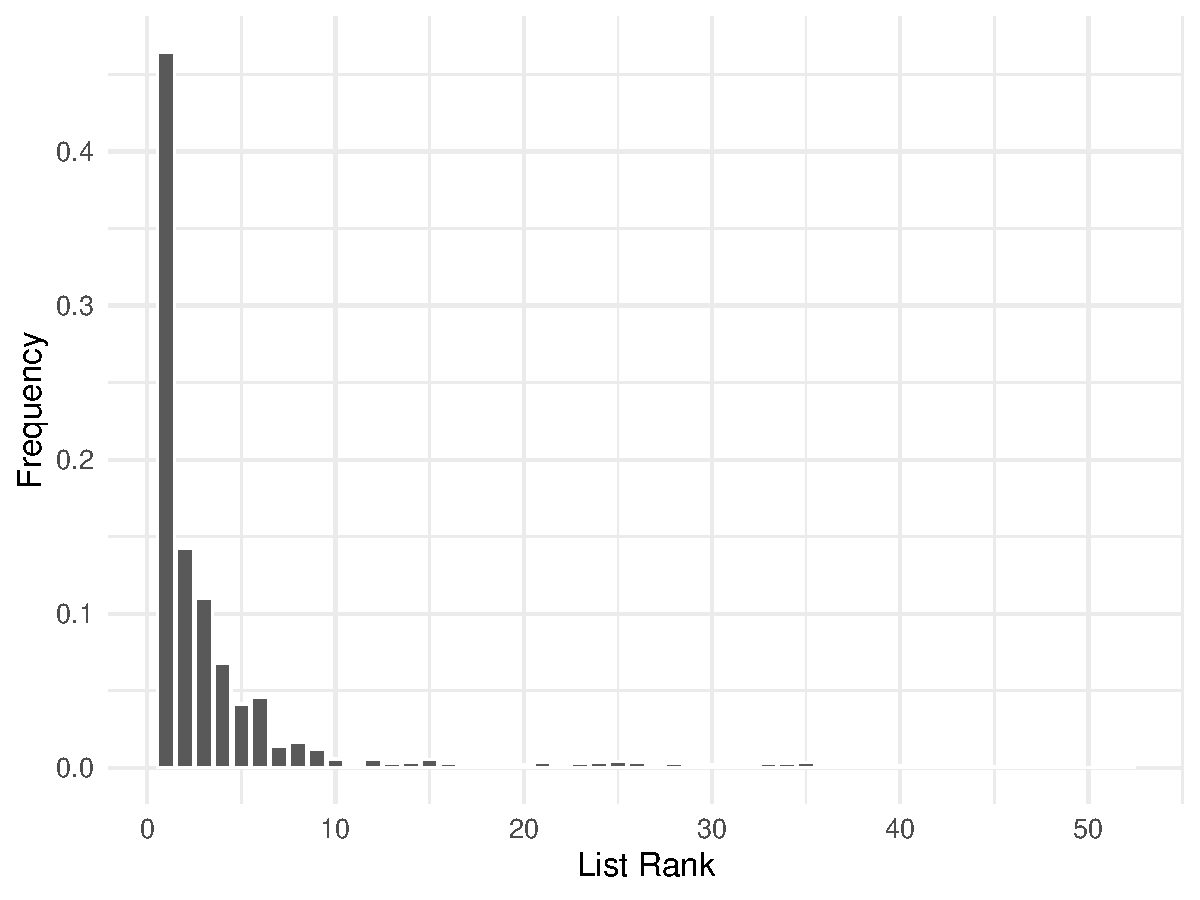
\includegraphics[width = 0.9\textwidth]{../figure/paper/pr_rank_distribution.pdf}
	\caption{Distribution of List Rank}
	\label{fig:distRank}
\end{figure}

\newpage

\subsection{Age of Winners}

\begin{figure}[!htbp]
	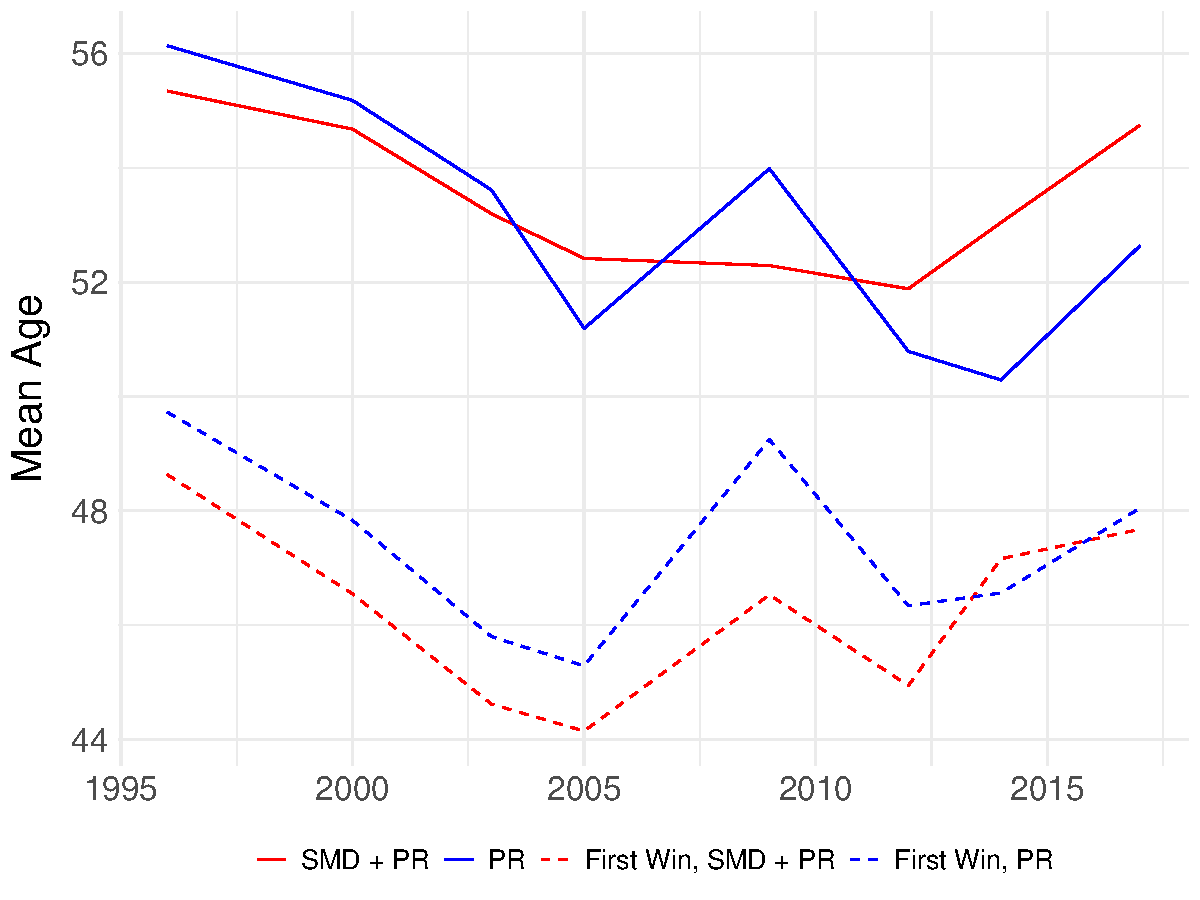
\includegraphics[width = 0.9\textwidth]{../figure/paper/age_first_win.pdf}
	\caption{Age Comparison: Average vs. New Legislators}
	\label{fig:ageFirstWin}
\end{figure}	

\newpage

\section{Additional Analyses}

\subsection{Aggregate-level Regression Table}


\begin{table}
\begin{center}
\begin{tabular}{l c c c c c c c c c c}
\hline
 & \multicolumn{4}{c}{List Rank} & \multicolumn{3}{c}{Dual Listing} & \multicolumn{3}{c}{Dual Listing (Tie)} \\
\cline{2-5} \cline{6-8} \cline{9-11}
 & Model 1 & Model 2 & Model 3 & Model 4 & Model 5 & Model 6 & Model 7 & Model 8 & Model 9 & Model 10 \\
\hline
Total Wins         & $-0.15^{***}$ &               &               & $-0.10^{***}$ & $0.16^{***}$ &              & $-0.00$      & $0.14^{***}$ &              & $0.00$        \\
                   & $(0.01)$      &               &               & $(0.02)$      & $(0.04)$     &              & $(0.02)$     & $(0.04)$     &              & $(0.02)$      \\
Incumbency         &               & $-1.02^{***}$ &               & $-0.74^{***}$ &              & $1.33^{***}$ & $1.33^{***}$ &              & $1.16^{***}$ & $1.13^{***}$  \\
                   &               & $(0.12)$      &               & $(0.11)$      &              & $(0.28)$     & $(0.28)$     &              & $(0.32)$     & $(0.31)$      \\
Dual Listing       &               &               & $-1.82^{***}$ & $-0.93^{***}$ &              &              &              &              &              &               \\
                   &               &               & $(0.25)$      & $(0.27)$      &              &              &              &              &              &               \\
Tie                &               &               &               & $-1.92^{*}$   &              &              &              &              &              &               \\
                   &               &               &               & $(0.86)$      &              &              &              &              &              &               \\
Female             &               &               &               & $-0.07$       &              &              & $-0.24^{*}$  &              &              & $-0.40^{***}$ \\
                   &               &               &               & $(0.04)$      &              &              & $(0.12)$     &              &              & $(0.11)$      \\
Block Magnitude    &               &               &               & $0.02^{***}$  &              &              & $0.04^{***}$ &              &              & $0.04^{***}$  \\
                   &               &               &               & $(0.01)$      &              &              & $(0.01)$     &              &              & $(0.01)$      \\
Total Wins x Tie   &               &               &               & $0.10^{***}$  &              &              &              &              &              &               \\
                   &               &               &               & $(0.02)$      &              &              &              &              &              &               \\
Tie x Incumbency   &               &               &               & $0.49^{**}$   &              &              &              &              &              &               \\
                   &               &               &               & $(0.18)$      &              &              &              &              &              &               \\
Tie x Dual Listing &               &               &               & $0.84$        &              &              &              &              &              &               \\
                   &               &               &               & $(0.91)$      &              &              &              &              &              &               \\
\hline
Year FE            & Yes           & Yes           & Yes           & Yes           & Yes          & Yes          & Yes          & Yes          & Yes          & Yes           \\
Party FE           & Yes           & Yes           & Yes           & Yes           & Yes          & Yes          & Yes          & Yes          & Yes          & Yes           \\
AIC                & $37167.39$    & $36446.03$    & $33098.42$    & $31652.57$    & $5886.23$    & $5697.89$    & $5629.09$    & $5949.29$    & $5803.79$    & $5729.36$     \\
Log Likelihood     & $-18536.69$   & $-18176.02$   & $-16502.21$   & $-15771.28$   & $-2897.12$   & $-2802.94$   & $-2765.54$   & $-2928.64$   & $-2855.90$   & $-2815.68$    \\
Num. obs.          & $7754$        & $7754$        & $7754$        & $7754$        & $7754$       & $7754$       & $7754$       & $7754$       & $7754$       & $7754$        \\
\hline
\multicolumn{11}{l}{\scriptsize{\item $^{***}p<0.001$; $^{**}p<0.01$; $^{*}p<0.05$. Standard errors clustered at the party level in parentheses.
\item Dependent variable: candidate $i$'s list rank (columns 1-4) dual listing status (columns 5-7), and whether the candidate has a tie on the list (columns 8-10).
\item Estimated models: negatige binomial (columns 1-4) and logit (columns 5-10).}}
\end{tabular}
\caption{Regression Results}
\label{tab:regression_results}
\end{center}
\end{table}


\newpage

\subsection{Party-level Analysis}

\subsubsection*{Komeito}


\begin{table}
\begin{center}
\begin{tabular}{l c c c c c c c c c c}
\hline
 & \multicolumn{4}{c}{List Rank} & \multicolumn{3}{c}{Dual Listing} & \multicolumn{3}{c}{Dual Listing (Tie)} \\
\cline{2-5} \cline{6-8} \cline{9-11}
 & Model 1 & Model 2 & Model 3 & Model 4 & Model 5 & Model 6 & Model 7 & Model 8 & Model 9 & Model 10 \\
\hline
Total Wins       & $-0.21^{***}$ &               &           & $-0.12^{***}$ & $0.32$   &          & $0.12$   & $0.34$   &          & $0.38$   \\
                 & $(0.02)$      &               &           & $(0.03)$      & $(0.19)$ &          & $(0.27)$ & $(0.24)$ &          & $(0.34)$ \\
Incumbency       &               & $-0.79^{***}$ &           & $-0.46^{***}$ &          & $1.50$   & $1.21$   &          & $1.17$   & $0.35$   \\
                 &               & $(0.07)$      &           & $(0.12)$      &          & $(0.88)$ & $(1.15)$ &          & $(1.25)$ & $(1.70)$ \\
Dual Listing     &               &               & $-0.26$   & $0.20$        &          &          &          &          &          &          \\
                 &               &               & $(0.23)$  & $(0.30)$      &          &          &          &          &          &          \\
Tie              &               &               &           & $-1.63$       &          &          &          &          &          &          \\
                 &               &               &           & $(1.96)$      &          &          &          &          &          &          \\
Female           &               &               &           & $-0.13$       &          &          & $-0.49$  &          &          & $1.06$   \\
                 &               &               &           & $(0.10)$      &          &          & $(1.19)$ &          &          & $(1.45)$ \\
Block Magnitude  &               &               &           & $0.04^{***}$  &          &          & $-0.06$  &          &          & $-0.05$  \\
                 &               &               &           & $(0.01)$      &          &          & $(0.06)$ &          &          & $(0.10)$ \\
Total Wins x Tie &               &               &           & $0.64$        &          &          &          &          &          &          \\
                 &               &               &           & $(0.71)$      &          &          &          &          &          &          \\
\hline
Year FE          & Yes           & Yes           & Yes       & Yes           & Yes      & Yes      & Yes      & Yes      & Yes      & Yes      \\
Party FE         & No            & No            & No        & No            & No       & No       & No       & No       & No       & No       \\
AIC              & $18.00$       & $1134.87$     & $1264.37$ & $1042.07$     & $57.30$  & $56.69$  & $61.28$  & $38.40$  & $39.19$  & $43.55$  \\
BIC              & $52.05$       & $1168.92$     & $1298.42$ & $1098.83$     & $87.57$  & $86.96$  & $102.91$ & $68.67$  & $69.46$  & $85.18$  \\
Log Likelihood   & $0.00$        & $-558.43$     & $-623.18$ & $-506.04$     & $-20.65$ & $-20.35$ & $-19.64$ & $-11.20$ & $-11.59$ & $-10.78$ \\
Deviance         & $180.36$      & $195.93$      & $309.02$  & $91.14$       & $41.30$  & $40.69$  & $39.28$  & $22.40$  & $23.19$  & $21.55$  \\
Num. obs.        & $325$         & $325$         & $325$     & $325$         & $325$    & $325$    & $325$    & $325$    & $325$    & $325$    \\
\hline
\multicolumn{11}{l}{\scriptsize{\item $^{***}p<0.001$; $^{**}p<0.01$; $^{*}p<0.05$. Standard errors in parentheses.
\item Dependent variable: candidate $i$'s list rank (columns 1-4) dual listing status (columns 5-7), and whether the candidate has a tie on the list (columns 8-10).
\item Estimated models: negatige binomial (columns 1-4) and logit (columns 5-10).}}
\end{tabular}
\caption{Regression Results for Komeito Candidates}
\label{tab:komeito}
\end{center}
\end{table}


\newpage

\subsubsection*{JCP}


\begin{table}[!htbp]
\begin{center}
\scalebox{0.7}{
\begin{threeparttable}
\begin{tabular}{l D{.}{.}{4.5} D{.}{.}{4.5} D{.}{.}{4.3} D{.}{.}{4.5} D{.}{.}{4.3} D{.}{.}{4.3} D{.}{.}{4.5} D{.}{.}{3.3} D{.}{.}{5.3} D{.}{.}{5.5}}
\toprule
 & \multicolumn{4}{c}{List Rank} & \multicolumn{3}{c}{Dual Listing} & \multicolumn{3}{c}{Dual Listing (Tie)} \\
\cmidrule(lr){2-5} \cmidrule(lr){6-8} \cmidrule(lr){9-11}
 & \multicolumn{1}{c}{Model 1} & \multicolumn{1}{c}{Model 2} & \multicolumn{1}{c}{Model 3} & \multicolumn{1}{c}{Model 4} & \multicolumn{1}{c}{Model 5} & \multicolumn{1}{c}{Model 6} & \multicolumn{1}{c}{Model 7} & \multicolumn{1}{c}{Model 8} & \multicolumn{1}{c}{Model 9} & \multicolumn{1}{c}{Model 10} \\
\midrule
Total Wins       & -0.22^{***}             &                         &                         & -0.10^{***}             & -0.03                   &                         & -0.04                   & -2.19^{*}               &                         & -1.40                   \\
                 & (0.02)                  &                         &                         & (0.03)                  & (0.05)                  &                         & (0.08)                  & (0.98)                  &                         & (1.13)                  \\
Incumbency       &                         & -0.95^{***}             &                         & -0.72^{***}             &                         & -0.12                   & -0.17                   &                         & -19.85                  & -17.22                  \\
                 &                         & (0.08)                  &                         & (0.11)                  &                         & (0.23)                  & (0.34)                  &                         & (2367.75)               & (2043.44)               \\
Dual Listing     &                         &                         & 0.07                    & -0.06                   &                         &                         &                         &                         &                         &                         \\
                 &                         &                         & (0.06)                  & (0.06)                  &                         &                         &                         &                         &                         &                         \\
Tie              &                         &                         &                         & -0.03                   &                         &                         &                         &                         &                         &                         \\
                 &                         &                         &                         & (0.11)                  &                         &                         &                         &                         &                         &                         \\
Female           &                         &                         &                         & 0.04                    &                         &                         & -0.12                   &                         &                         & -0.99^{*}               \\
                 &                         &                         &                         & (0.05)                  &                         &                         & (0.21)                  &                         &                         & (0.46)                  \\
Block Magnitude  &                         &                         &                         & 0.05^{***}              &                         &                         & 0.07^{***}              &                         &                         & 0.13^{***}              \\
                 &                         &                         &                         & (0.00)                  &                         &                         & (0.01)                  &                         &                         & (0.04)                  \\
Total Wins x Tie &                         &                         &                         & 0.29                    &                         &                         &                         &                         &                         &                         \\
                 &                         &                         &                         & (0.51)                  &                         &                         &                         &                         &                         &                         \\
\midrule
Year FE          & \multicolumn{1}{c}{Yes} & \multicolumn{1}{c}{Yes} & \multicolumn{1}{c}{Yes} & \multicolumn{1}{c}{Yes} & \multicolumn{1}{c}{Yes} & \multicolumn{1}{c}{Yes} & \multicolumn{1}{c}{Yes} & \multicolumn{1}{c}{Yes} & \multicolumn{1}{c}{Yes} & \multicolumn{1}{c}{Yes} \\
Party FE         & \multicolumn{1}{c}{No}  & \multicolumn{1}{c}{No}  & \multicolumn{1}{c}{No}  & \multicolumn{1}{c}{No}  & \multicolumn{1}{c}{No}  & \multicolumn{1}{c}{No}  & \multicolumn{1}{c}{No}  & \multicolumn{1}{c}{No}  & \multicolumn{1}{c}{No}  & \multicolumn{1}{c}{No}  \\
AIC              & 1775.10                 & 1750.64                 & 1897.57                 & 1568.00                 & 628.43                  & 628.60                  & 610.54                  & 178.03                  & 180.35                  & 162.47                  \\
BIC              & 1820.69                 & 1796.23                 & 1943.16                 & 1638.45                 & 669.87                  & 670.04                  & 664.42                  & 219.48                  & 221.79                  & 216.34                  \\
Log Likelihood   & -876.55                 & -864.32                 & -937.78                 & -767.00                 & -304.21                 & -304.30                 & -292.27                 & -79.02                  & -80.18                  & -68.23                  \\
Deviance         & 385.60                  & 372.88                  & 423.51                  & 191.69                  & 608.43                  & 608.60                  & 584.54                  & 158.03                  & 160.35                  & 136.47                  \\
Num. obs.        & 466                     & 466                     & 466                     & 466                     & 466                     & 466                     & 466                     & 466                     & 466                     & 466                     \\
\bottomrule
\end{tabular}
\begin{tablenotes}[flushleft]
\scriptsize{\item $^{***}p<0.001$; $^{**}p<0.01$; $^{*}p<0.05$. Standard errors in parentheses.
\item Dependent variable: candidate $i$'s list rank (columns 1-4) dual listing status (columns 5-7), and whether the candidate has a tie on the list (columns 8-10).
\item Estimated models: negatige binomial (columns 1-4) and logit (columns 5-10).}
\end{tablenotes}
\end{threeparttable}
}
\caption{Regression Results for JCP Candidates}
\label{tab:jcp}
\end{center}
\end{table}


\end{document}































